Bei einem „teile und herrsche“-Ansatz wird das eigentliche Problem so lange in kleinere und einfachere Teilprobleme zerlegt, bis man diese\linebreak lösen („beherrschen“) kann. Anschließend wird aus diesen Teillösungen eine Lösung für das Gesamtproblem (re-)konstruiert.
\subsubsection{Anwendung}
„Teile und herrsche“ \,ist eines der \,wichtigsten Prinzipien für effiziente Algorithmen. Dabei wird ausgenutzt, dass bei vielen Problemen der Aufwand sinkt, wenn man das Problem in kleinere Teilprobleme zerlegt. Dies lässt sich meist durch Rekursive Programmierung umsetzen, bei der die Teilprobleme wie eigenständige Probleme gleichzeitig parallel oder sequenziell (einzeln nacheinander) behandelt werden, bis sie auf triviale Lö\-sungen zurückgeführt sind oder der \, Restfehler hinreichend klein ist. Bei manchen Algorithmen steckt dabei die Kernidee im Schritt des „Teilens“, während die „Rekombination“ einfach ist (beispielsweise Quicksort). In anderen \linebreak Verfahren (beispielsweise Mergesort) ist das Teilen einfach, während die Rekombination die Kernidee des Algorithmus enthält. In manchen Algorithmen sind beide Schritte komplex.
\footnote[1]{Wikipedia zu D\&C}
\subsection{Arithmetik großer Zahlen}
In der Schule hat man bereits einen oder mehrere Algorithmen gelernt um die Grundrechenarten auf beliebige Zahlen an zu wenden. Hier sollen nun weitere vorgestellt werden.

Als Beispiel für große Arithmetische Operationen kann unter anderem die RSA angeführt werden. Speziell in Programmiersprachen wie C trifft man auf Rundungsprobleme, die abgefangen werden müssen. Hier verlässt man sich oft nicht auf die eingebaute Arithmetik und entwickelt eigene (zuweilen schnellere) Lösungsansätze.

\subsubsection{Addition}
Nehmen wir nun zwei Zahlen und addieren sie wie früher in der Schule\\
\begin{tabular}{lllllllll}
&3&4&2&7&6&5&1\\
+& &$2_1$&$6_1$&$4_1$&4&3&2\\\hline
&3&6&9&2&0&8&3
\end{tabular}\\
%$$3427651+264432=3692083$$
Da Zahlen in verschiedensten Zahlensystemen benutzt und dargestellt werden können, von Binär über Dezimal bis hin zu beliebigen Basen, möch\-ten wir eine gute allgemeingültige\, Darstellung wählen.
Eine beliebige Zahl kann zu jeder Basis folgendermaßen dargestellt werden:
\begin{align*}
A=\sum_{i=0}^{n-1} a_i b^i &:& 0\le a_i<b\\
C=\sum_{i=0}^{n-1} c_i b^i &:& 0\le c_i<b
\end{align*}
Der oben angesprochene Algorithmus hat mit der darauffolgenden Datenstruktur die Laufzeit $$T(n)=c*n$$
\subsubsection{Multiplikation}
Nehemen wir hier nun zwei Binärzahlen: \\[.5em]
\begin{figure}[H]\center\begin{tabular}{l@{ }l@{ }l@{ }l@{ }l@{ }l@{ }l@{ }l@{ }l@{ }l@{ }l@{ }l@{ }l@{ }l@{ }l@{ }l@{ }l}
1&0&1&0&1&1&0&1&0&$\bullet$&1&1&1&1&0&0&1\\
&&&&&&&&A&$\bullet$&&&&&&&C\\
\\
&&1&0&1&0&1&1&0&1&0&.&.&.&.&.&.\\
&+&&1&0&1&0&1&1&0&1&0&.&.&.&.&.\\
&+&&&1&0&1&0&1&1&0&1&0&.&.&.&.\\
&+&&&&1&0&1&0&1&1&0&1&0&.&.&.\\
&+&&&&&0&0&0&0&0&0&0&0&0&.&.\\
&+&&&&&&0&0&0&0&0&0&0&0&0&.\\
&+&&&&&&&1&0&1&0&1&1&0&1&0\\\hline
&&&&&&..&1&1&1&0&0&0&1&0&1&0
\end{tabular}
\caption{Binäre Multiplikation}
\end{figure}
Dieser Algorithmus kann mathematisch folgendermaßen aufgefasst werden:
\begin{align*}
=&AB\\=&\left(\sum_{i=0}^{n-1} a_i b^i\right)\left(\sum_{j=0}^{n-1} c_j b^j\right)\\=&\sum_{i=0}^{n-1}\sum_{j=0}^{n-1}  a_i c_j b^{i+j}
\end{align*}
Die Schulmultiplikation hat eine Laufzeit von\linebreak $T(n)=c*n^2$. Dies bedeutet für große Zahlen, z.B. $$n=10^6 \Rightarrow T(n)=10^{12}$$
Dies kostet uns sehr viel Zeit. Das die Addition schneller geht zeigte uns der Student Karazuba\footnote{Paper von Karazuba und Offman}.
\subsubsection{Erster Ansatz mit D\&C}

Wir haben Zwei Zahlen $A$ und $C$ von welchen wir je die vordere und die Hintere hälfte nehmen. 
\begin{figure}[H]
\center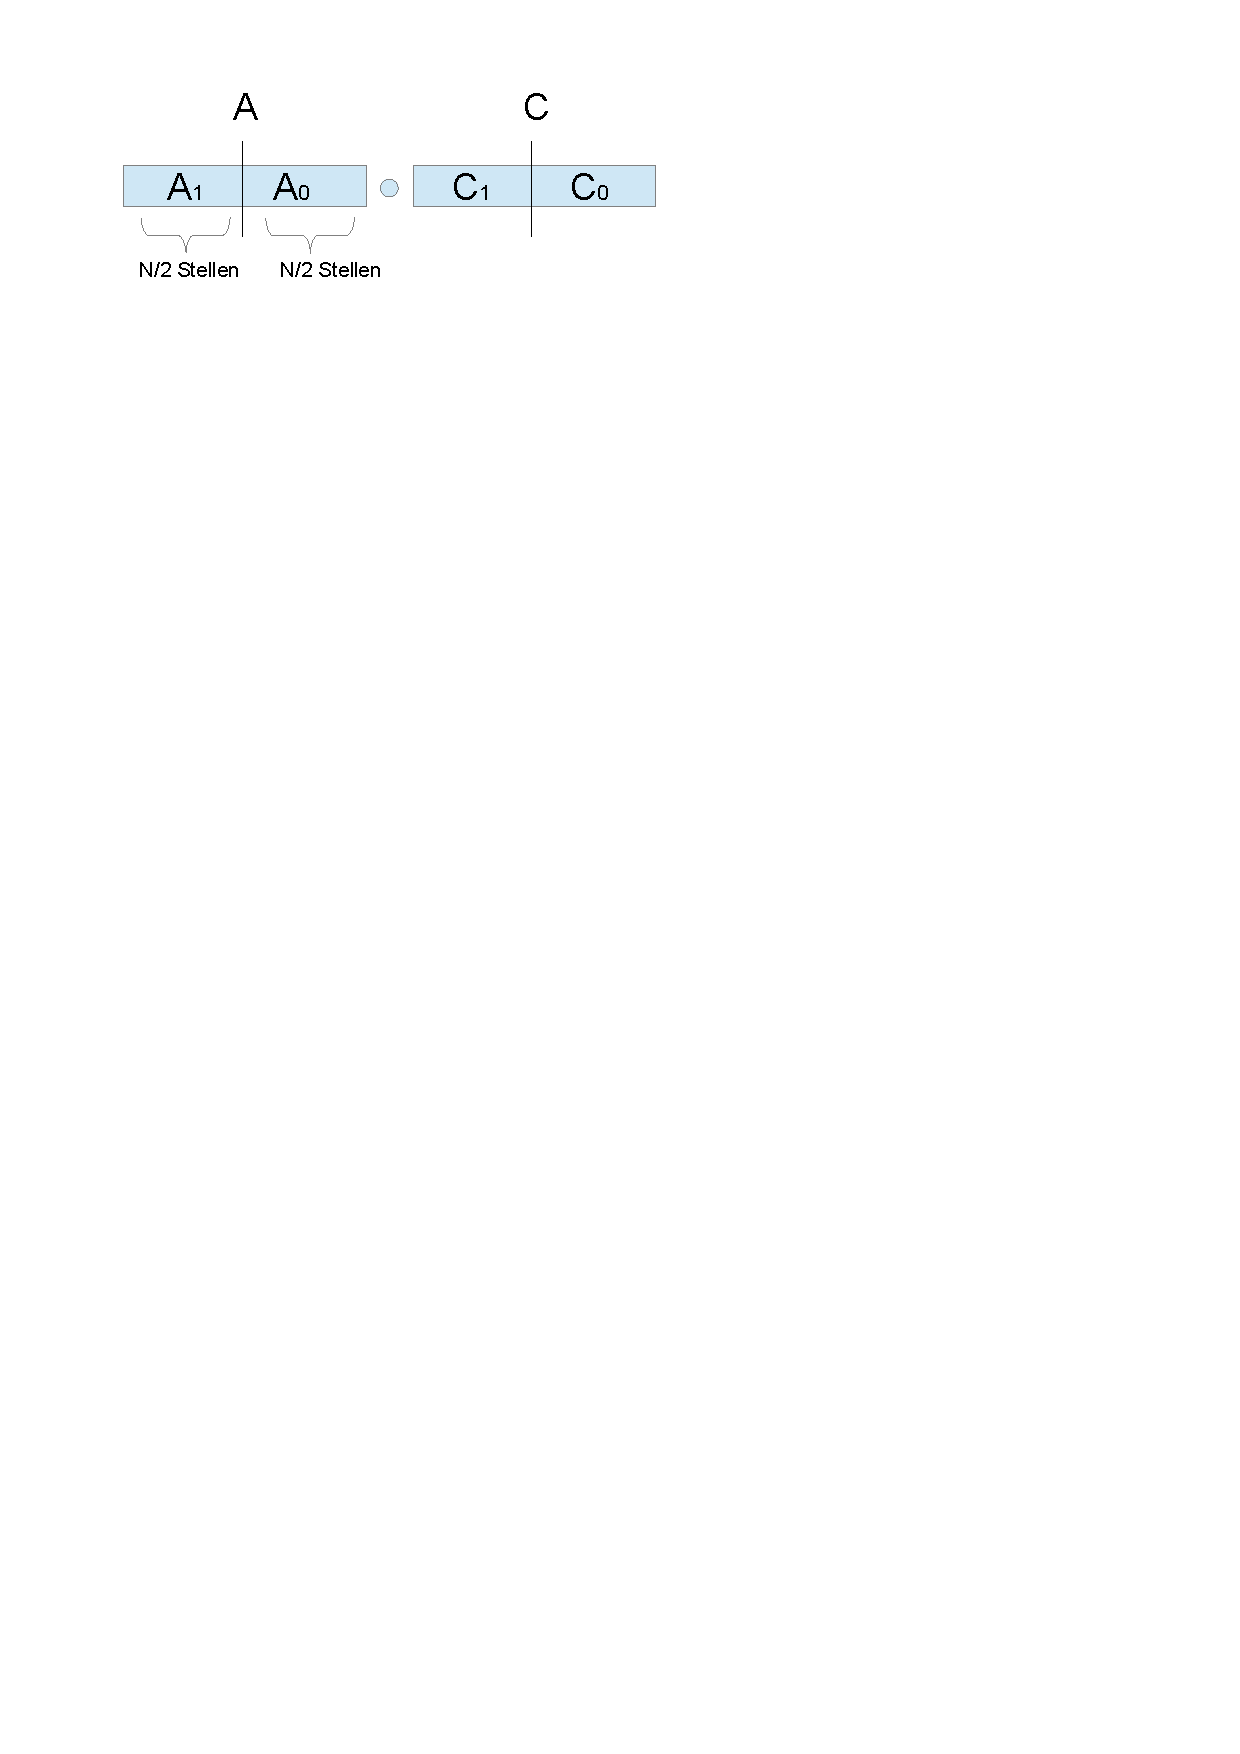
\includegraphics[trim= 2cm 25cm 9.5cm 1.5cm,clip,width=\columnwidth]{figures/DundC.pdf}
\caption{Divide and Conquer bei zwei Feldern}
\end{figure}
Damit ergeben sich folgende Rechenschritte
\begin{align*}
A&=\sum_{i=0}^{n-1} a_i b^i = A_i b^{\frac{n}{2}}+A_0\\
A_0&=\sum_{i=0}^{\frac{n}{2}-1} a_i b^i\\
A_1&=\sum_{i=0}^{\frac{n}{2}-1} a_{i+\frac{n}{2}} b^i\\
\end{align*}
$b^n$ stellt einen binären Shift dar. Wenn wir nun A in zwei Hälften teilen, ist der vordere Teil ($A_1$) um $b^\frac{n}{2}$ voneinander verschoben.
\begin{eqnarray*}
A=123456;&C=987654\\
A\bullet C&\\
A_1=123;&C_1=987\\
A_0=456;&C_2=654\\
A_1b^\frac{n}{2}+A_0=A\\
123000+456&=123456
\end{eqnarray*}
Hier ist der binäre Shift gut zu erkennen. Wie auch die Addition hat der Binärshift linearen \linebreak Aufwand.

Das Produkt $AC$ kann man nun auch folgendermaßen ausdrücken
\begin{align*}
AC&=(A_1b^{\frac{n}{2}}+A_0)(C_1b^{\frac{n}{2}}+C_0)\\
&=A_1C_1b^n+A_1C_0b^{\frac{n}{2}}\\
&\qquad {}+A_0C_1b^\frac{n}{2}+A_0C_0
\end{align*}
Indem das Problem auf diese Art immer weiter vereinfacht wird, überführe ich das quadratische Problem in viele Additionen mit linearem Aufwand.

Betrachten wir uns nun die Laufzeit des Algorithmus. 
\begin{align*}
T(n)&=4T\left(\frac{n}{2}\right)+cn\\
T(1)&=c
\end{align*}
Dies nennt man eine \textbf{Rekursionsgleichung}!

Eine solche R. sagt nur bedingt etwas über die Laufzeit aus. Hierzu muss man diese Gleichung lösen und ggf. mit Induktion o.Ä. lösen.
Bei Betrachtung der Glieder der rekursiven Folge erhalten wir
\begin{align*}
T(n)&=4^kT\left(\frac{n}{2^k}\right)+cn\sum_{i=0}^{k-1}2^i\\
&=4^kT\left(\frac{n}{2^k}\right)+cn\left(2^k-1\right)\\
\mbox{mit}\log_2n:\\
T(n)&=4^{\log_2n}T(1)+cn\left(2^{\log_2n}-1\right)\\
&=n^2c+cn\left(n-1\right)\\
&\le2cn^2
\end{align*}
Wie man hier sieht, hat auch diese Methode einen quadratischen Aufwand. 

\subsection{Karazuba}
Karazuba hatte die Idee, die Zahl der Teilprodukte von vier auf drei zu minimieren.

Dazu stellen wir das D\&C Produkt $AC$ um.
\begin{align*}
AC&=A_0C_1b^{\frac{n}{2}}+A_1C_0b^{\frac{n}{2}}+A_1C_1b^n+A_0C_0\\
&=\left(A_0C_1+A_1C_0\right)b^{\frac{n}{2}}+A_1C_1b^n+A_0C_0\\
&=P_3b^{\frac{n}{2}}+P_2b^n+P_1
\end{align*}
Wenn wir uns nun die drei Produkte einzeln ansehen ist die Vereinfachung schnell zu erkennen
\begin{align*}
P_1&=A_0C_0\\
P_2&=A_1C_1\\
P_3&=A_0C_1+A_1C_0\\
&=(A_1C_1+A_1C_0+A_0B1+A_0B_0)\\
&\qquad {}-A_1C_1-A_0C_0\\
&=\left((A_1+A_0)(C_1+C_0)\right)-P_2-P_1
\end{align*}
denn man sieht, dass man bei $P_3$ nur noch ein Produkt rechnen muss und die anderen beiden Produkte zur Korrektur mittels Multiplikation\linebreak und damit konstantem Aufwand in die Rechnung einfließen.

Bei der Frage an das Auditorium, wie hoch nun die Laufzeit sei, gab es die folgende\\[.5em]
\textbf{Behauptung}
$$T_K(n)=cn^{\log_23}$$
\begin{figure}[h]
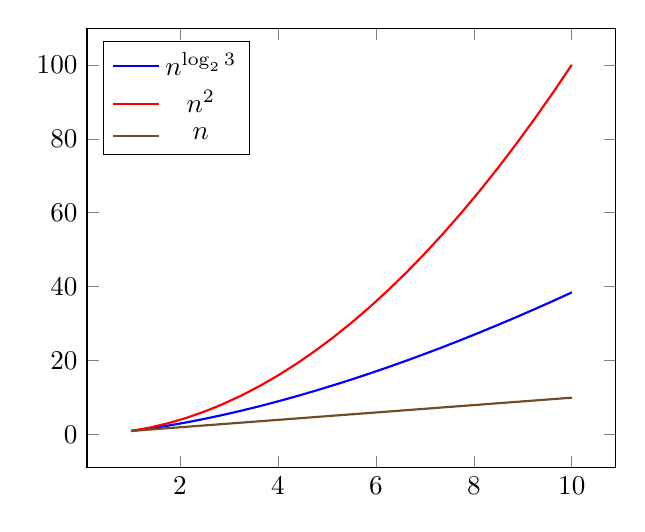
\begin{tikzpicture}[scale=.98]
\begin{axis}[legend pos=north west,legend entries={$n^{\log_23}$,$n^2$,$n$}]
\addplot+[no markers,domain=1:10,thick]{x^1.58496};
\addplot+[no markers,domain=1:10,thick]{x^2};
\addplot+[no markers,domain=1:10,thick]{x};
\end{axis}
\end{tikzpicture}
\caption{Laufzeit Multiplikation}
\end{figure}
Hier ist schön zu sehen, um wie viel niedriger der Aufwand im Gegenzug zu $n^2$ ausgefallen ist. Nachfolgend ein kleines Beispiel mit einer\linebreak Größenordnung von 6 für $n$.
\begin{align*}
n&=10^6\\
n^2&=10^{12}\\
n^{\log_23}=n^{1,58\ldots}&\approx10^{9}
\end{align*}

Normalerweise wird erwartet dass der Verlauf eines effizienteren Algorithmuses folgendermaßen verläuft, wobei man gut erkennen kann, dass der effizientere Algorithmus erst ab einem bestimmten n effizienter ist, als der naive Ansatz.
\begin{figure}[H]
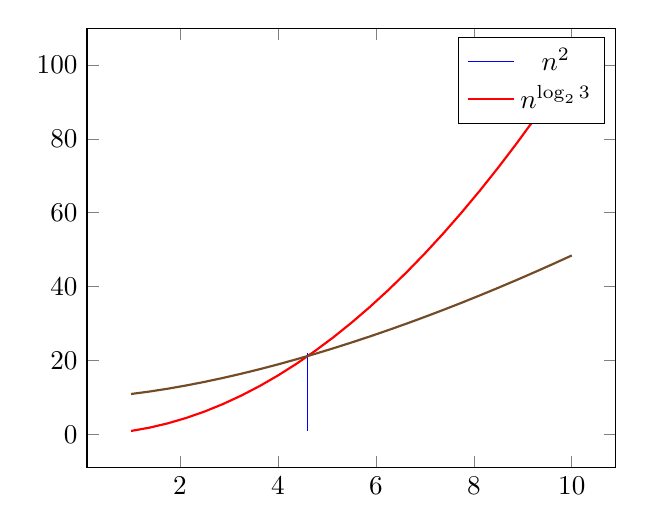
\begin{tikzpicture}[scale=.98]
\begin{axis}[legend entries={$n^2$,$n^{\log_23}$}]
\addplot+[no markers] coordinates {(4.61,22) (4.61,1)};
\addplot+[no markers,domain=1:10,thick]{x^2};
\addplot+[no markers,domain=1:10,thick]{(x^1.58496)+10};
\end{axis}
\end{tikzpicture}
\caption{Laufzeit est. Break-even Point}
\end{figure}

Wie verhällt sich nun die Laufzeit für die doppelte Menge an Eingabedaten?
\begin{align*}
\frac{T_S(2n)}{T_S(n)}&=\frac{c(2n)^2}{c(n)^2}&=4\\
\frac{T_K(2n)}{T_K(n)}&=frac{c(2n)^{\log_23}}{c(n)^{\log_23}}&=3
\end{align*}

Gut zu sehen ist, dass sich der Aufwand bei Verdopplung des Naiven vervierfacht und er sich bei K. nur verdreifacht.
\subsection{Schnelle Matrizenmultiplikation nach Strassen}

wir nehmen zwei Matrizen $A,B\in \mathbb R^{n\times n}$ und\linebreak führen auf diesen eine Multiplikation aus.
\begin{align*}C&=AB\\
c_{ij}&=\sum_{k=1}^na_{ik}b_{kj} &1\le i,j \le n\\
\end{align*}
deren Aufwand
$$T(n)=cn^3$$
entspricht.
\[\left(\begin{array}{c@{ }|c@{ }}
A_{1,1} & A_{1,2} \\\hline
A_{1,1} &A_{2,2}
\end{array}\right)\left(\begin{array}{c@{ }|c@{ }}
B_{1,1} & B_{1,2} \\\hline
B_{1,1} &B_{2,2}
\end{array}\right)=\left(\begin{array}{c@{ }|c@{ }}
C_{1,1} & C_{1,2} \\\hline
C_{1,1} &C_{2,2}
\end{array}\right)\]
$$A_{1,1},A_{1,2},A_{2,1},A_{2,2}\in \mathbb R^{\frac{n}{2}\times\frac{n}{2}}$$
\begin{align*}
C_{1,1}&=A_{1,1}B_{1,1}+A_{1,2}B_{2,1}\\
C_{1,2}&=\ldots\\
&\vdots\\
C_{2,2}&=
\end{align*}
Der Aufwand ist hier nun
\begin{align*}T(n)&=8T\left(\frac{n}{2}\right)+cn^2\\
T(1)&=c
\end{align*}
Wenn man diese Rekursionsgleichung löst erhält man für den Aufwand $$T(n)=c^3$$
Hier kommt nun wieder Karazubas Idee ins Spiel den Aufwand von acht zu sieben zu minimieren.

Dies geschieht folgendermaßen:\\
Hab ich keine Lust zu...\\
Daraus folgt
$$\Rightarrow T(n)=7T\left(\frac{n}{2}\right)+cn^2$$
Die Lösung hiervon, werden wir nun mit Hilfe des Mastertheorems ausrechnen, welches wir uns nach der Zusammenfassung herleiten wollen.